\section{Quirks}\label{sec:quirks}
\begin{multicols}{2}
\begin{ffcolpage}
Quirks are characteristics that define your character's personality and/or backstory. They give the player some tips on how to roleplay their character and are a tool both to earn Destiny Points and to use them. Some Quirk also got a keyword. You may not have more than one quirk with the same keyword, so you can't be Caustic and Empathic at the same time. And absolutely no Half-Viera/Half-Elvaan, please! \pc

Destiny Points are a shared group resource that may be used to give the players some control in the narrative. They may be used to turn a failed Challenge into a successful one, to give tips and directions, to perform heroic actions that surpass human capacity and even to cheat death, among various other uses. Details on how to earn and how to spend Destiny Points are on the Game Engine Chapter, starting at page~\pageref{ch:characters}.
\end{ffcolpage}

\subsection{Quirk List}\label{subsec:quirklist}

\begin{ffcolpage}
\tquirk{Arrogant}: You don’t back off from challenges and don’t submit to the will of others. You may spend Destiny Points to resist intimidation. However, you do not take insults lightly and don’t refuse challenges. Earn Destiny Points when this attitude causes you problems.
\end{ffcolpage} \pw

\begin{ffcolpage}
\begin{wrapfigure}{l}{0.35\textwidth}
    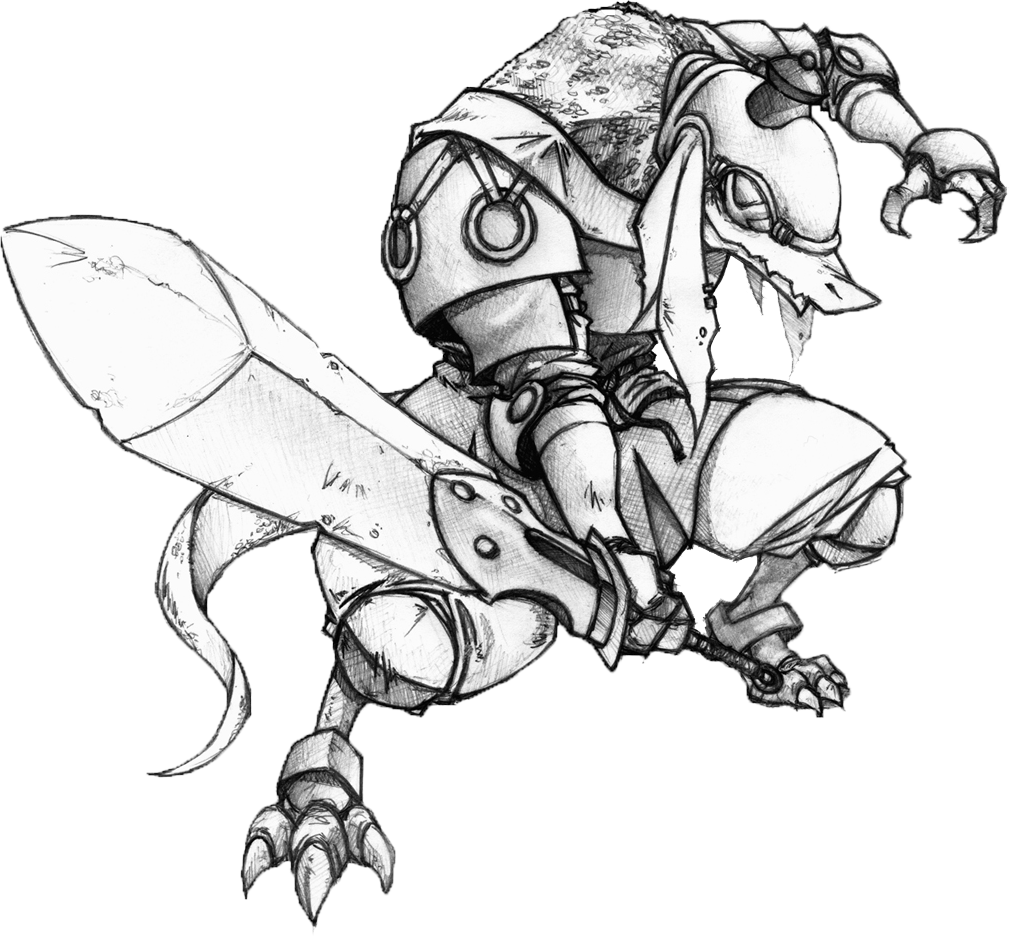
\includegraphics[width=0.3\textwidth]{race-bangaa}
\end{wrapfigure}
\tquirk{Bangaa (racial)}: A people of biped lizard men. They are as tall as humans, but significantly stronger and covered with hard scales. You may use Destiny Points due to your great strength, leathery skin and high strength to overcome physical Challenges. However, your race has a terrible vision and it is not uncommon for Bangaa to cover their eyes to focus only on hearing and smell. Although you can still see, but the lack of an accurate vision may cause you problems, and if that happens, earn Destiny Points.
\end{ffcolpage} \pw

\begin{ffcolpage}
\tquirk{Bottomless Pockets}: You usually have everything always at hand. Spend Destiny Points to find things you did not expect, as that wrench you were just looking for! However, sometimes you simply won’t find something you were sure that were with you. When this causes you problems, earn Destiny Points.
\end{ffcolpage} \pw

\begin{ffcolpage}
\tquirk{Brute (body)}: You are very strong and heavy. Spend Destiny Points to overcome challenges whenever your muscle power really makes a difference. However, your weight and lack of reflexes can cause you problems, granting you Destiny Points.
\end{ffcolpage} \pw

\begin{ffcolpage}
\tquirk{Caustic (charisma)}: You attract dislike and people feel uncomfortable by your side. You may use Destiny Points to intimidate or otherwise impose your will on others. You receive Destiny Points when this lack of sympathy causes you problems.
\end{ffcolpage} \pw

\begin{ffcolpage}
\tquirk{Contacts}: You have contacts to obtain information or favors. Decide at character creation what kind of contacts you have and what kind of favors they would be willing to do. To use these favors, spend Destiny Points. However, your contacts may ask dangerous favors or cause you problems, granting you Destiny points.
\end{ffcolpage} \pw

\begin{ffcolpage}
\tquirk{Compulsive Liar (honesty)}: For some reason, telling the truth is very hard for you. Worse, others believe! Use Destiny Points to make people believe your lies, especially the most ridiculous, and earn Destiny Points whenever your lack of honesty causes you problems.
\end{ffcolpage} \pw

\begin{ffcolpage}
\begin{wrapfigure}{r}{0.35\textwidth}
    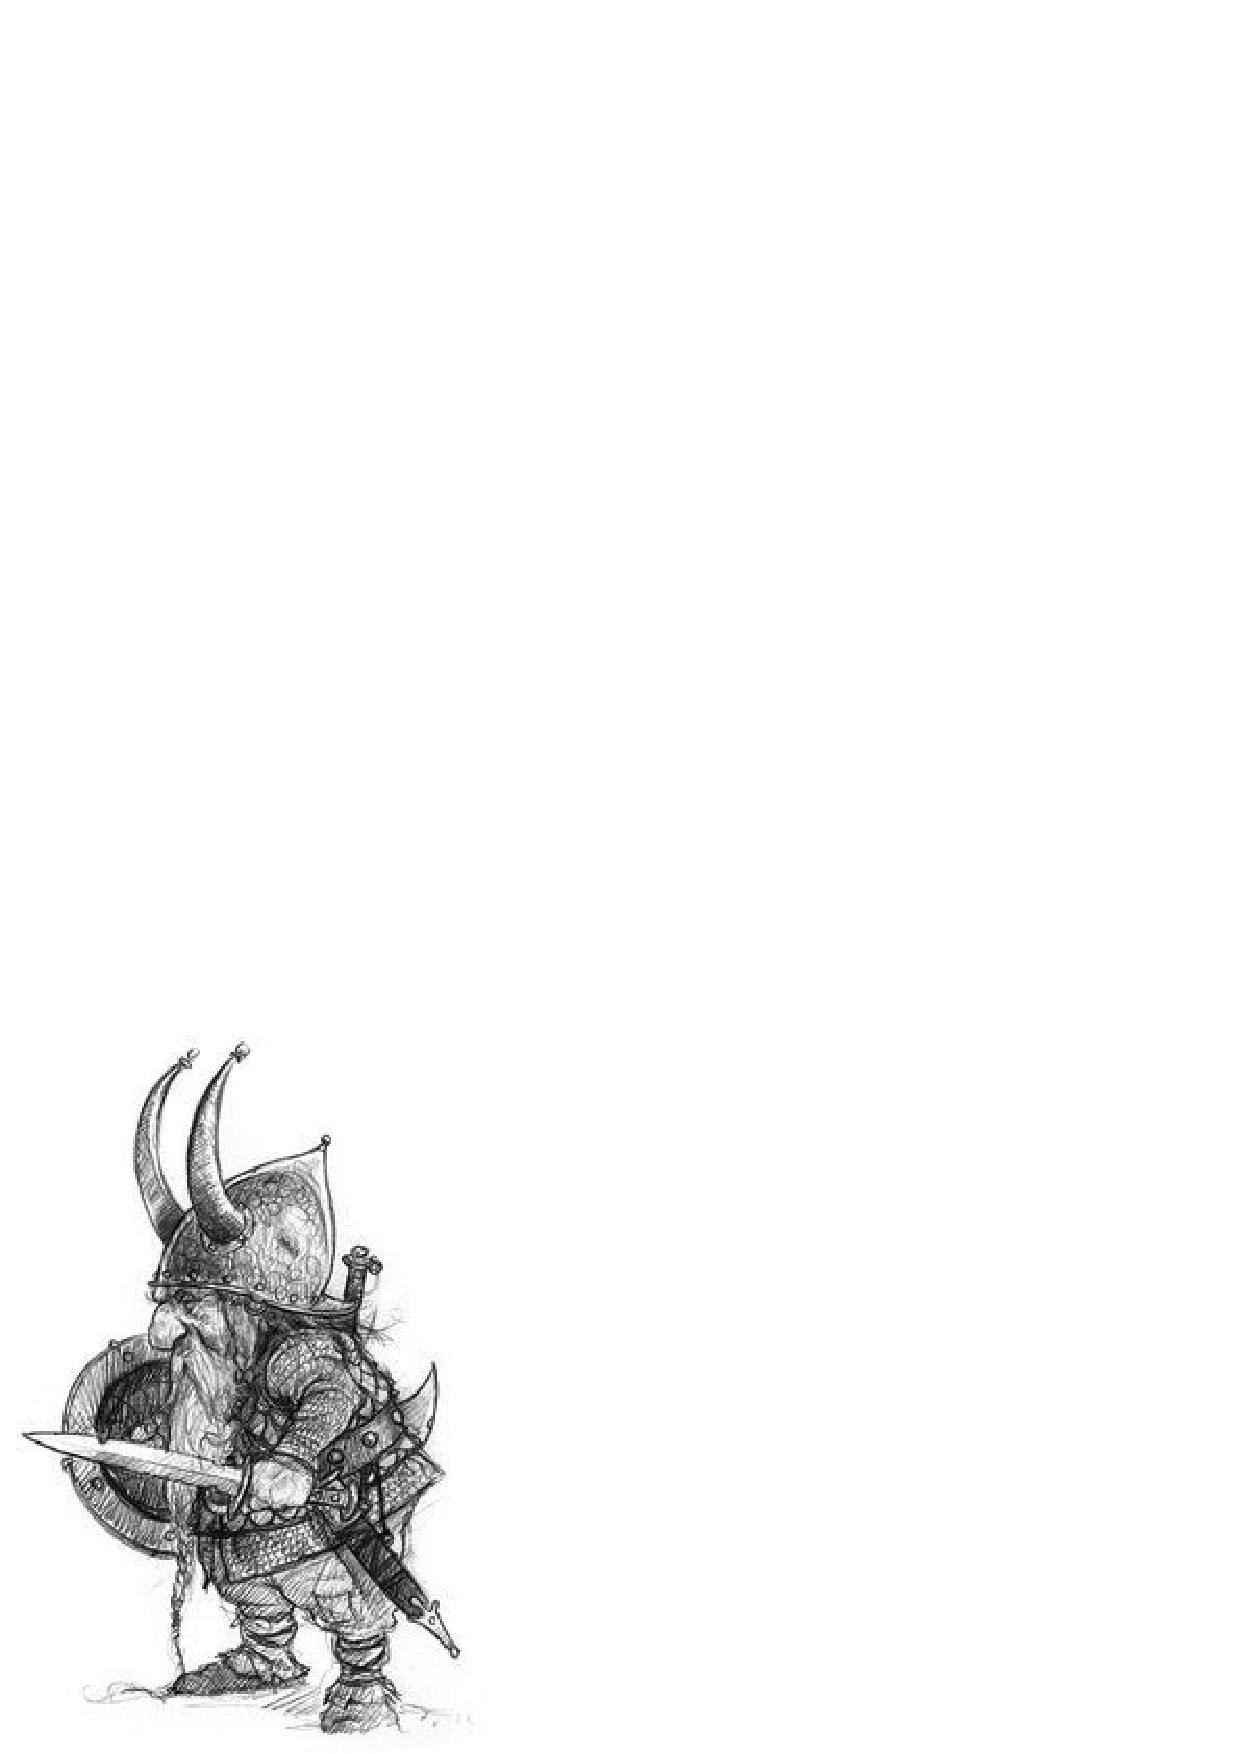
\includegraphics[width=0.3\textwidth]{race-dwarf}
\end{wrapfigure}
\tquirk{Dwarf (racial)}: Creatures that live underground in caves and mines, building great kingdoms and castles under the rock. They are generally smaller and more muscular than humans, possessing an innate aptitude for metallurgy and technology. You may use Destiny Points in situations involving explosives, machinery and mining, activities for which dwarves are renowned. However, the time spent in the darkness turns sunlight into an ongoing discomfort, making you feel bad in bright light. Whenever this causes you problems, earn Destiny Points.
\end{ffcolpage} \pw

\begin{ffcolpage}
\begin{wrapfigure}{l}{0.35\textwidth}
    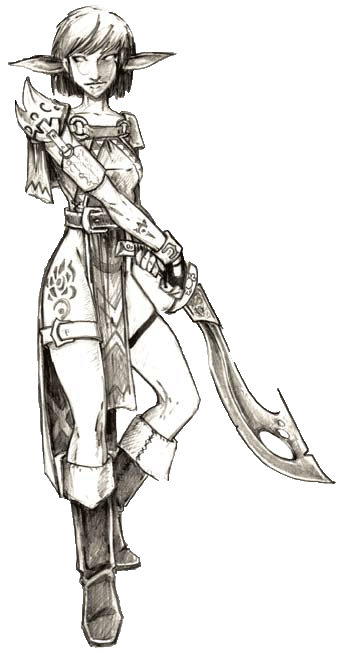
\includegraphics[width=0.3\textwidth]{race-elvaan}
\end{wrapfigure}
\tquirk{Elvaan (racial)}: Proud, athletic, slender and towering, Elvaan are known for their prominent pointed ears, often stretching ten to fifteen centimeters to the sides of their heads. Some call them the Elves or Elezen. You may use Destiny Points in situations that require courage, confidence and willpower. However, Elvaan are famous for their arrogance and inability to forgive offenses, whether real or imagined. Whenever this causes you problems, earn Destiny Points.
\end{ffcolpage} \pw

\begin{ffcolpage}
\tquirk{Empathic (charisma)}: You attract sympathy and people feel comfortable at your side. You may use Destiny Points to attract sympathy and good impressions. However, people tend to not take you seriously. If this causes you problems, earn Destiny Points.
\end{ffcolpage} \pw

\begin{ffcolpage}
\tquirk{Fast (body)}: You are fast and light. Spend Destiny Points to use your speed to your advantage but earn Destiny Points when your lack of strength or resistance causes you problems.
\end{ffcolpage} \pw

\begin{ffcolpage}
\tquirk{Feral (animal)}: You were raised by beasts, monsters or a savage tribe. You relate well with animals. Use Destiny Points to attract animal sympathy and calm them. However, you are unable to get along with other humans and earn Destiny Points whenever that causes you problems.
\end{ffcolpage} \pw

\begin{ffcolpage}
\tquirk{Focused}: You are focused on some issues (decide which). Unfortunately, this leaves you with little regard for other subjects. You may use Destiny Points to remember specific knowledge of your studies. Earn Destiny Points when your lack of attention to other matters causes you problems.
\end{ffcolpage} \pw

\begin{ffcolpage}
\tquirk{Intuitive Magic – Elemental}: You can spend Destiny Points to manipulate fire, lightning and ice, creating small magical effects. Your magical skills, however, can’t be used in combat. Sometimes, magic does not work the way or when you want, and if this causes you problems, earn Destiny Points.
\end{ffcolpage} \pw

\begin{ffcolpage}
\tquirk{Intuitive Magic – Forces}: You can spend Destiny Points to telekinetically manipulate objects, as well as air, earth and water, performing small magical effects. Your magical skills, however, can’t be used in combat. Sometimes, magic does not work the way or when you want, and if this causes you problems, earn Destiny Points.
\end{ffcolpage} \pw

\begin{ffcolpage}
\tquirk{Intuitive Magic – Illusion}: You can spend Destiny Points to manipulate lights, shadows and illusions, performing small magical effects. Your magical skills, however, can’t be used in combat. Sometimes, magic does not work the way or when you want, and if this causes you problems, earn Destiny Points.
\end{ffcolpage} \pw

\noindent\begin{ffcolpage}
\begin{wrapfigure}{r}{0.35\textwidth}
    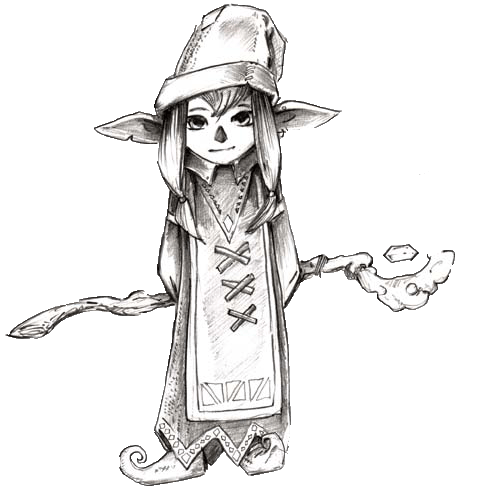
\includegraphics[width=0.3\textwidth]{race-lalafell}
\end{wrapfigure}
\tquirk{Lalafell (racial)}: These little creatures are among the smallest known races, hardly reaching more than a meter tall. In their own language, they call themselves Tarutaru. You may spend Destiny Points to make small magical effects by manipulating telekinetically objects as well as to control light and shadows. Their magical skills, however, can’t be used in combat. Their small stature and lack of physical strength can cause problems when they try to overcome situations that require strength and endurance. Whenever this happens, earn Destiny Points.
\end{ffcolpage} \pw

\begin{ffcolpage}
\tquirk{Lycanthrope}: Your senses are much more acute than usual. You can use Destiny Points to track by scent or discover things that only your keen senses would find. But his bestial blood tries to take control of you, and you have a constant internal struggle to not act like an animal. Whenever this cause problems, earn Destiny Points.
\end{ffcolpage} \pw

\begin{ffcolpage}
\begin{wrapfigure}{l}{0.35\textwidth}
    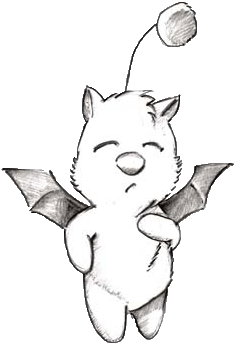
\includegraphics[width=0.3\textwidth]{race-moogle}
\end{wrapfigure}
\tquirk{Moogle (racial)}: Their appearance is similar to a humanoid cat, usually white in color, with small wings of red or purple color and an antenna on his head ending in a red ball (pompom). Their ears are like those of a cat or a dog. Despite having wings, they can't fly, but their pompoms give almost telepathic abilities with other moogle, building what some scholars call Mognet. You may spend Destiny Points to gather information or send messages through Mognet to other moogle. However, their spoken language heavily depends on the kupo word, which can have several meanings depending on the intonation and body movements. Because of this, communication with other races is full of misunderstandings. Whenever this causes you problems, earn Destiny Points.
\end{ffcolpage} \pw

\begin{ffcolpage}
\tquirk{Naive Idealist}: You see life through the lens of a personal code of conduct, or some religious fanaticism, or an ideological utopia. Either way, you're very attached to that ideals, and you can draw strength from them. The details of your ideal code must be fleshed out with the GM, but you can spend Destiny points to face incredible odds when adhering to it. However, you're gullible and easily manipulable, as your ideals may be used to cause you problems, earning you Destiny Points.
\end{ffcolpage} \pw

\begin{ffcolpage}
\tquirk{Natural Hunter (animal)}: You feel more comfortable away from civilization. Forests are your second home. You can use Destiny Points to hunt, seek shelter and track in natural environments. However, you are already so used to kill animals that they avoid you and feel uncomfortable around you. If this causes you problems, earn Destiny points.
\end{ffcolpage} \pw

\begin{ffcolpage}
\tquirk{Nu Mou (racial)}: They have similarities with dogs, with elongated snouts, furry tails and big, floppy, ears. Their short stature, around a meter and a half tall, and their tendency to a stooped posture, cause them to be very small. They have a fragile constitution, but they are very intelligent and tend to live three times more than normal humans. You may use Destiny Points in situations involving patience, common sense and obscure knowledge, especially magical knowledge. They are also slow and not very athletic. Whenever this causes you problems, earn Destiny Points.
\end{ffcolpage} \pw

\begin{ffcolpage}
\tquirk{Paranoid}: You're always aware of the dangers that can arise at any time. Spend Destiny Points to perceive things that only your keen senses may notice. However, you suspect everyone and everything, and if this causes you problems, earn Destiny Points.
\end{ffcolpage} \pw

\begin{ffcolpage}
\begin{wrapfigure}{r}{0.35\textwidth}
    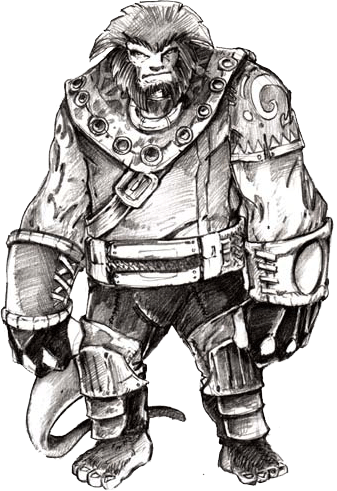
\includegraphics[width=0.3\textwidth]{race-roegadyn}
\end{wrapfigure}
\noindent\tquirk{Roegadyn (racial)}: Also known as Galka, this race with slightly ursine appearance has huge bodies, often over two meters tall. Despite their great strength and power, they are renowned for self-knowledge and phlegm. You may use Destiny Points in situations involving self-control and great physical strength. But often their overly calm attitude may look like apathy or simply laziness. Whenever this causes you problems, earn Destiny Points. \pw
\end{ffcolpage}

\begin{ffcolpage}
\noindent\tquirk{Straight Arrow (honesty)}: You're a straight arrow, rarely lie and got a reputation for honesty. You may spend Destiny Points to make people believe and trust you. Earn Destiny points whenever your honesty causes you problems.
\end{ffcolpage} \pw

\begin{ffcolpage}
\noindent\tquirk{Uncommon Beauty}: You are very beautiful and can use your beauty to attract attention and get good impressions. You may use Destiny Points to influence other characters who would feel attracted to you. Whenever your beauty causes you problems, earn Destiny Points.
\end{ffcolpage} \pw

\begin{ffcolpage}
\begin{wrapfigure}{l}{0.35\textwidth}
    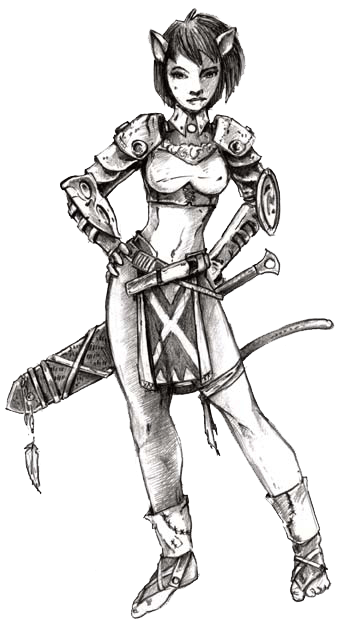
\includegraphics[width=0.3\textwidth]{race-viera}
\end{wrapfigure}
\noindent\tquirk{Viera (racial)}: The Viera have two sub-races. The most common live in temperate forests and has long rabbit ears, but there is a sub-race that lives in tropical jungles and has feline characteristics rather than rabbit’s. This sub-breed is commonly called Mithra or Miqo'te. Regardless of the sub-race, they are mostly female, with males being only about twenty percent of the population. Moreover, they are closely linked to the forests and jungles where they live. You may use Destiny Points to communicate with trees, although their cognitive ability is very limited. On the other hand, you feel extremely uncomfortable in urban environments, and can even become ill if you stay away from the natural environment for a long time. Whenever this causes you problems, earn Destiny Points. \pw
\end{ffcolpage}

\begin{ffcolpage}
\tquirk{Visions}: For some reason, you have visions that can give you tips of the future or just torture you. Spend Destiny Points for good visions and earn Destiny Points when flashbacks cause you trouble.
\end{ffcolpage} \pw

\begin{ffcolpage}
You may also want to create your own Quirks. Choose a trait that defines your character and talk with your GM to turn into a Quirk. However, there are three guidelines that should be followed. First, a Quirk must be able to provide the player ways to spend Destiny Points to overcome Challenges; second, a quirk must be able to provide the GM ways to create problems for the group; and lastly, a quirk may not influence tactical combat rolls.
\end{ffcolpage}
\end{multicols}

\section{Stats and Skills}\label{sec:stats}
\begin{multicols}{2}
\subsection{Stats}\label{subsec:stats}
Characters have four Stats, each connected to a crystal --- Earth, Air, Fire and Water. Each Stat has a value and levels. For every 10 points in its value, the Stat earns another level. Stat's value varies from 0 to 255 and, consequently, between 0 and 25 levels. The sum of a character’s Stat levels is his Character level. \pc

For example, a 30th level character may have Earth 52 (5th level), Air 108 (10th level), Fire 80 (8th level) and Water 75 (7th level). Each Stat has 6 skills associated to it. The sum of all Skill levels a character has in all skills linked to a particular Stat may not be higher than its Stat level. Thus, the above character has 10 points to spend in all skills but may not spend more than 5 points in Earth skills, no more than 8 points in Fire skills and no more than 7 points in Water Skills. \pc

Stats are also used in the tactical combat system. Each roll in combat uses one Offensive and one Defensive Stat. Earth is usually the Offensive Stat for attacks that depends on the user's brute force and physicality and is the Defensive Stat to attacks that may be prevented by the defender's physical strength, health and
muscle power. \pc

Attacks that rely on the user's speed, finesse and skill use Air as its Offensive Stat. It is the Defensive Stat against attacks that may be evaded by the defender's reflexes and agility. A primarily Offensive Stat, Fire is used in attacks that rely on the user's intelligence and magical ability. If an attack may be avoided by the defender's insight, it uses Fire as it Defensive Stat. \pc

Lastly, attacks that depends on the user's charisma and willpower to hit uses Water as its Offensive Stat. However, it is a mainly Defensive Stat, as attacks that may be resisted by the user's mental strength and magical defenses should use it. Besides its offense and defense implications, players should note that your Earth Value is added to your hit points (HP) and your Water Value is added to your magic points (MP) value. \pc

Stats are increased using experience points. The cost to increase a Stat's value by a single point is one plus twice the Stat level. Thus, a Stat costs 1 experience point per Stat point while at level 0 (value from 0 to 9); 3 experience points per Stat point while at level 1 (value 10 to 19); 5 XP per Stat point while at level 2 (value 20 to 29); and so on. Starting on page 125, there is a table with the total XP cost for each Stat value. \pc
{\centering %
    \adjincludegraphics[width=.5\textwidth-2\columnsep]{block-crystalparty}%
}%

\subsection{Skills}\label{subsec:skills}
\begin{ffcolpage}
Skills are tools that the characters have to overcome Challenges. Each Challenge must relate to a Skill. Each Skill level means the player may re-roll once a Challenge related to that Skill. For example, a character with 3 levels in Strength Skill can re-roll the d100 3 times to overcome Strength Challenges. \pc

Earth Skills involve brute strength, toughness, physical prowess and bulk. A character's Earth level is his limit to spend points in \tskill{Strength}, \tskill{Climbing}, \tskill{Swimming}, \tskill{Intimidation}, \tskill{Tolerance}, or \tskill{Jumping}. \pc

Air Skills involve movement, finesse and body coordination. A character's Air level is his limit to spend points in \tskill{Running}, \tskill{Stealth}, \tskill{Piloting}, \tskill{Riding}, \tskill{Thievery}, or \tskill{Acrobatics}. \pc

Fire Skills involve intelligence, knowledge and wisdom. A character's Fire level is his limit to spend points in \tskill{Infiltration}, \tskill{Perception}, \tskill{Medicine}, \tskill{Survival}, \tskill{Technology}, or \tskill{Wisdom}. \pc

Water Skills involve willpower and charisma. A character's Water level is his limit to spend points in \tskill{Willpower}, \tskill{Bluff}, \tskill{Handle Animal}, \tskill{Charisma}, \tskill{Performance}, or \tskill{Magic}.
\end{ffcolpage} \pc
Below is a description of each Skill and examples of Challenges associated with them. \pw

\begin{ffcolpage}
\tskill{Acrobatics} (Air): Ability to perform acrobatic maneuvers and maintain balance in difficult situations. Can be used in situations where the character may lose balance, must walk on cliffs or wires, or in situations where it hangs on masts, chandeliers or ropes.
\end{ffcolpage} \pw

\begin{ffcolpage}
\tskill{Bluff} (Water): Ability to lie, cheat, conceal and seduce. It can be used in situations to deceive, pretend, or otherwise attempt to conceive your true intentions.
\end{ffcolpage} \pw

\begin{ffcolpage}
\tskill{Charisma} (Water): Personal magnetism and ability to impress. It can be used in situations involving the reactions of non-player characters, sometimes even without any specific action by the character.
\end{ffcolpage} \pw

\begin{ffcolpage}
\tskill{Climbing} (Earth): Climbing speed and technique. It can be used in situations that involve climbing walls, mountains, trees and other obstacles.
\end{ffcolpage} \pw

\begin{ffcolpage}
\tskill{Handle Animal} (Water): Ability to soothe and train animals and monsters. It can be used in situations requiring empathy with animals, to calm wildlife, train animals or prevent them from attacking someone.
\end{ffcolpage} \pw

\begin{ffcolpage}
\tskill{Infiltration} (Fire): Ability to open locks and gain access to locked locations. It can include both the ability to unlock locks with lock picks as the ability to fake access cards in more modern environments.
\end{ffcolpage} \pw

\begin{ffcolpage}
\tskill{Intimidation} (Earth): Ability to impose your will through coercion, threats and power displays. It can be used in situations where the character wants to impose its will in the most direct way possible.
\end{ffcolpage} \pw

\begin{ffcolpage}
\tskill{Jumping} (Earth): Jumping capacity, involving both the distance as the height. It can be used in situations involving the ability to overcome pits or to reach high platforms.
\end{ffcolpage} \pw

\begin{ffcolpage}
\tskill{Magic} (Water): Knowledge of arcane magic. It can be used in situations involving knowledge of the magical forces of the world and its mysteries.
\end{ffcolpage} \pw

\begin{ffcolpage}
\tskill{Medicine} (Fire): Knowledge of anatomy, healing, herbal medicines and medical techniques. It can be used in various situations involving diseases, poisonings and remedies.
\end{ffcolpage} \pw

\noindent\parbox{.15\textwidth}{
    \adjincludegraphics[width=.15\textwidth]{skill-performance}
}\begin{minipage}{.35\textwidth-1\columnsep}
\tskill{Perception} (Fire): Ability to distinguish detail with the five senses. It can be used in situations involving sight, hearing, smell, touch or
taste. 
\par\pw
\tskill{Performance} (Water): Ability to act, sing, dance, or perform other forms of art. It can be carried out in situations involving artistic performances, such as an opera.
\end{minipage}
\pw

\begin{ffcolpage}
\tskill{Piloting} (Air): Ability to drive inanimate machines, ranging from chariots and carriages to giant robots and aircraft, depending on the setting’s technology.
\end{ffcolpage} \pw

\begin{ffcolpage}
\tskill{Riding} (Air): Ability to ride animals such as chocobos. It can be used in situations involving the ability to ride animals, in pursuits or to do mounted maneuvers.
\end{ffcolpage} \pw

\begin{ffcolpage}
\tskill{Running} (Air): Ability to walk and run fast and for long distances. It can be used in situations involving the running speed and endurance in long distance runs.
\end{ffcolpage} \pw

\begin{ffcolpage}
\tskill{Stealth} (Air): Ability to hide and move silently. It can be used in situations when the character doesn’t want to be noticed.
\end{ffcolpage} \pw

\begin{ffcolpage}
\tskill{Strength} (Earth): Strength and physical ability. It can be used in situations involving the character's ability to lift, pull, push and knock down things.
\end{ffcolpage} \pw

\begin{ffcolpage}
\tskill{Survival} (Fire): Ability to relate to the natural world and get food, water and shelter outdoors. It can be used in situations where the character needs to hunt and gather food and water in wild environments.
\end{ffcolpage} \pw

\begin{ffcolpage}
\tskill{Swimming} (Earth): Ability to cross distances by swimming. It can be used in situations involving the need to cross rivers, lakes, seas, or simply to avoid drowning.
\end{ffcolpage} \pw

\begin{ffcolpage}
\tskill{Technology} (Fire): Ability to relate to existing technology on the world, varying according to the setting’s technology level. It can vary from gear-operated primitive machines to the operation and maintenance of sophisticated computers.
\end{ffcolpage} \pw

\begin{ffcolpage}
\tskill{Thievery} (Air): Ability to perform hands tricks, as making small objects exchange owner without anyone noticing. It can be used in situations involving theft, traps or sleight of hand.
\end{ffcolpage} \pw

\begin{ffcolpage}
\tskill{Tolerance} (Earth): Ability to resist hot and cold environments, hunger, thirst, drowning and suffocation. It can be used in situations where the character must overcome physical hardships.
\end{ffcolpage} \pw

\begin{ffcolpage}
\tskill{Willpower} (Water): Ability to resist intimidation, pain, suffering and torture. It can be used to withstand suffering and to endure the physical and emotional hardships.
\end{ffcolpage} \pw

\begin{ffcolpage}
\tskill{Wisdom} (Fire): Common sense and the ability to distinguish illusions, tricks and deceptions. It can be used in situations that require the character’s judgment to avoid being fooled.
\end{ffcolpage}
\end{multicols}
